\documentclass[xelatex,ja=standard,jafont=noto]{bxjsarticle}
\usepackage[utf8]{inputenc}

\usepackage{amsmath}
\usepackage{amsthm}
\usepackage{amssymb}
\usepackage{mathrsfs}
\usepackage{graphicx} 
\usepackage{braket}


\newtheorem{theorem}{Theorem}
\newtheorem{corollary}{Corollary}
\newtheorem{lemma}{Lemma}
\newtheorem{example}{Ex\documentclass{article}
	\usepackage{CJKutf8}
	\usepackage{amsmath}
	\usepackage{amsthm}
	\usepackage{amssymb}
	ample}
\newtheorem{definition}{Definition}

\def\ds{\displaystyle}
\def\ul{\underline}
	\title{量子力学の理論と数学}
	\author{bq18026\\関宇}
	\date{12.10,2020}
	
	
\begin{document}
\maketitle

\section{}

\subsection{条件付き確率}

ある事象が起こるという条件の下で考える確率を条件付き確率という.事象$B$が起こる条件のもとで、事象Aが起こる条件付き確率${\rm Pr}(A|B)$は、

\begin{equation}
    Pr(A|B)=\frac{Pr(A\cap B)}{Pr(B)}
\end{equation}
で定義される.ここで、分子はAかつBが起こる確率、Pr(B)はBを起こる確率.したがって、$Pr(\ket{\psi})$を(状態$\ket{\psi}$を準備する確率)、$Pr(A=a\cap\ket{\psi})$を(状態が$\ket{\psi}$でかつAの測定値がaとなる確率)とすると、

\begin{equation}
    \bra{\psi}P_{a}\ket{\psi}=Pr(A=a|\ket{\psi})=\frac{Pr(A=a\cap\ket{\psi})}{Pr(\ket{\psi})}
\end{equation}

\subsection{周辺分布}
$Pr(A=a,B=b|\ket{\psi})$のように複数出力を持つ場合、一つの出力のみに着目した確率分布を周辺分布と呼ぶ.周辺分布は、確率の和法則より、着目している出力以外の確率を全て足すことにより求められる.例えば、Aの周辺分布は
\begin{equation}
    \sum_{b}Pr(A=a,B=b|\ket{\psi})
\end{equation}
あらゆる状態$\ket{\psi}$の下で、同時確率分布の周辺分布が、
\begin{equation}
    \begin{aligned}
        &\bra{\psi}Pa\ket{\psi}=\sum_{b}Pr(A=a,B=b|\ket{\psi})\\
        \\
        &\bra{\psi}Qb\ket{\psi}=\sum_{a}Pr(A=a,B=b|\ket{\psi})
    \end{aligned}
\end{equation}

\begin{center}
\begin{tabular}{ |c|c|c|c| } 
 \hline
 a/b & 0 & 1 & marginal distribution of A\\ 
 \hline
 0 & 1/4 & 1/4 & 1/2\\ 
 \hline
 1 & 1/4 & 1/4 & 1/2\\ 
 \hline
 marginal distribution of B & 1/2 & 1/2 &  1 \\ 
 \hline
\end{tabular}
\end{center}

\newpage

\subsection{凸集合と凸関数}
実ベクトル空間$V$の任意の二つの要素$v_{1},v_{2}\in V,p\in [0,1]$に対して、$pv_{1}+(1-p)v_{2}$で表わさVの要素をpについて凸結合という.特に、Vの部分集合Wで任意の二つの要素$w_{1},w_{2}\in W,p\in [0,1]$について凸結合$pw_{1}+(1-p)w_{2}$がWに含まれるとき、凸(部分)集合と呼ばれる.幾何学的には、凸集合はへこみのない部分集合である.\\

\begin{figure}[h!]
    \centering
    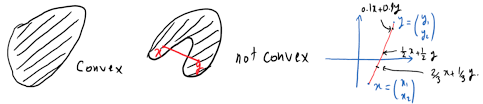
\includegraphics[scale=0.7]{1.png}
    \caption{convex combination}
\end{figure}
密度演算子の集合は凸集合である.特に、凸集合Wの元wが非自明な凸結合を持たない時、wは端点(extreme point)と呼ばれる.すなわち、$w_{1},w_{2}\in W,p\in(0,1)$に対して、$w=pw_{1}+(1-p)w_{2}$が成り立つならば、$w=w_{1}=w_{2}$である.幾何学的には、端点は凸集合の角である.d個の事象について確率分布の集合において、端点は1......dのうちのどれか一つの事象が確率1で起きる確率分布のみである.また、純粋状態は密度演算子からなる凸集合の端点である.\\

二つの凸集合W,Vが与えられ、 WからVへの写像fが以下の条件を満たすとき、(すなわち凸結合を保存する時)fはアフィンであるという.
\begin{equation}
    f(pw_{1}+(1-p)w_{2})=pf(w_{1})+(1-p)f(w_{2})
\end{equation}
次に、凸集合W確率分布実数$\mathcal{R}$への写像fが以下の条件を満たすとき、fは凸関数であるという.
\begin{equation}
    f(pw_{1}+(1-p)w_{2})\leqq pf(w_{1})+(1-p)f(w_{2})
\end{equation}
特に、ある$0<p<1$について等号が成り立つのは$w_{1}=w_{2}$に限られるとき、fは狭義凸関数(strictly convex function)であるという.\\

\newpage

命題4.4.4

    $\rho SE$を$\mathcal{H}_{SE}$上の密度演算子とすると、その部分トレース$\rho s:=Tr_{E}\rho SE$は$\mathcal{H}_{s}$上の密度演算子である.\\
    
    証明:
    
    演習問題24(3)より、$\rho s$の正値性が成り立つ.
    
    \begin{equation}
        \begin{aligned}
            Tr \rho s&=\sum_{i}\bra{\psi_{i}}\rho s\ket{\psi_{i}}\\
            \\
            &=\sum_{i,k}\bra{\psi_{i}\otimes e_{k}}C\ket{\psi_{i}\otimes e_{k}}\\
            \\
            &=Tr_{SE}\rho SE=1
        \end{aligned}
    \end{equation}
    
密度演算子$\rho s:=Tr_{E}\rho SE$を$\rho SE$の縮約密度演算子と呼ぶ.\\


命題4.4.5

全体系S+E系の状態が」密度演算子$\rho SE$で記述されるとき、S系の縮約状態は縮約密度演算子$\rho s:=Tr_{E}\rho SE$で与えられる.\\

証明:

Sの縮約状態を対応する密度演算子を$\sigma s$とする.S上の任意の物理量$A=\sum_{a}aP_{a}$の測定を考える.

この物理量はS+E上で
\begin{equation}
    A\otimes I_{E}=\sum_{a}a(P_{a}\otimes I_{E})
\end{equation}
で記述されるので、


\begin{equation}
    Pr(A=a|\sigma s)=Tr_{SE}(P_{a}\otimes I_{E}\rho SE)
\end{equation}

演習問題24(2)より、

\begin{equation}
    Tr_{SE}(P_{a}\otimes I_{E}\rho SE)=Tr_{S}(P{a}(Tr_{E}\rho SE))
\end{equation}

さらに,Bornの確率規則より、

\begin{equation}
    Tr_{S}(P{a}(Tr_{E}\rho SE))=Pr(A=a|\rho s)\ket{\phi}\bra{\psi}
\end{equation}
となる.Aは任意なので、$\sigma S=\rho S$を得る.\\


\section{純粋化}

あらゆる混合状態は、合成系上の純粋状態に帰着できる.すなわち、系Sの状態が混合状態であったとしても、ある補助系Aを考えることで、Sの状態を合成系S+A上の純粋状態$\rho SA$の縮約状態とすることができるのである.これを状態の純粋化と呼ぶ.


\section{同時測定}
同時測定とは、あらゆる状態の下で、


\end{document}
